

\chapter{Prototype System}
We have so far introduced our conceptual model for reactive \textrm{\glspl{infosystem}} and their Services and some example use cases to point out what would be possible with our model.
In this chapter we present our proof of concept prototype system, which has a focus on the Web as its \textrm{\gls{infospace}}.
We will then introduce our \textrm{\acrshort{eca}} rule language, which gives all the necessary power over our prototype system and which can be directly translated into the internal rules representation.



\section{Architecture}
The prototype system is the adoption of our conceptual model for reactive \textrm{\glspl{infosystem}} and their services to the Web.
The Web consists of many \textrm{\glspl{infosystem}} and because of its \textrm{\acrlong{soa}} it can be seen as one large \textrm{\gls{infosystem}}, therefore we can impose reactivity on the Web.
Since communication over services in the Web is often latency driven, we came to the conclusion that asynchronous communication and therefore scalability should be attributes our prototype system has to support natively.
Another aspect to be regarded for the architectural decision was how the rules are going to be represented internally.
We introduced \textrm{\acrshort{xml}} and \textrm{\acrshort{json}} as common ways to communicate data between services on the Web.
Both formats represent data in a tree structure, and this is also what we decided to assume for the explicit parameters in the events that will enter our prototype.
Together with the requirement of native support for an \textrm{\acrlong{eda} (\acrshort{eda})} our decision was to build upon the recent adoption of \textrm{JavaScript} to application development through \textrm{Node.js}\footnote{http://nodejs.org/} and its human-readable \textrm{\acrshort{json}} communication format.

The prototype system consists of several modules, shown in Figure \ref{fig:Architecture}, which we are going to introduce within this section:
\begin{itemize}
	\item \textbf{\textrm{Poller}:} Loads \textrm{Event Trigger} modules and forwards events coming from them to the \textrm{Event Queue}. \textrm{Event Trigger} modules poll for changes in the Web and transform them into events. 
	\item \textbf{\textrm{\gls{webhook} Listener}:} Listens on active \textrm{\gls{webhook}} for events and forwards them to the \textrm{Event Queue}.
	\item \textbf{\textrm{Event Queue}:} Buffers events for the case of an overly busy \textrm{Rule Engine}. 
	\item \textbf{\textrm{Rules Engine}:} Picks an event from the \textrm{Event Queue} whenever there is one and it is idle. 
	\item \textbf{\textrm{User Request Handler}:} The user interface modules to administrate \textrm{Event Triggers}, \textrm{\gls{webhook}}, \textrm{Rules} and \textrm{Action Dispatchers}.
\end{itemize}

When started, the prototype system loads persisted \textrm{\gls{webhook}} and begins to listen for new events on them.
The \textrm{Rule Engine} then loads all persisted rules and for each rule it loads the required \textrm{Action Dispatchers} and notifies the \textrm{Poller} about the new rule, which in turn loads an \textrm{Event Trigger} if required.
The prototype is now up and running and accepts administration requests for \textrm{Event Triggers}, \textrm{\gls{webhook}}, \textrm{Rules} and \textrm{Action Dispatchers}.
Whenever a rule is created or updated, the \textrm{Poller} and \textrm{Rule Engine} load required \textrm{Event Triggers} or \textrm{Action Dispatchers}.

\begin{figure}[!ht]
	\centering
  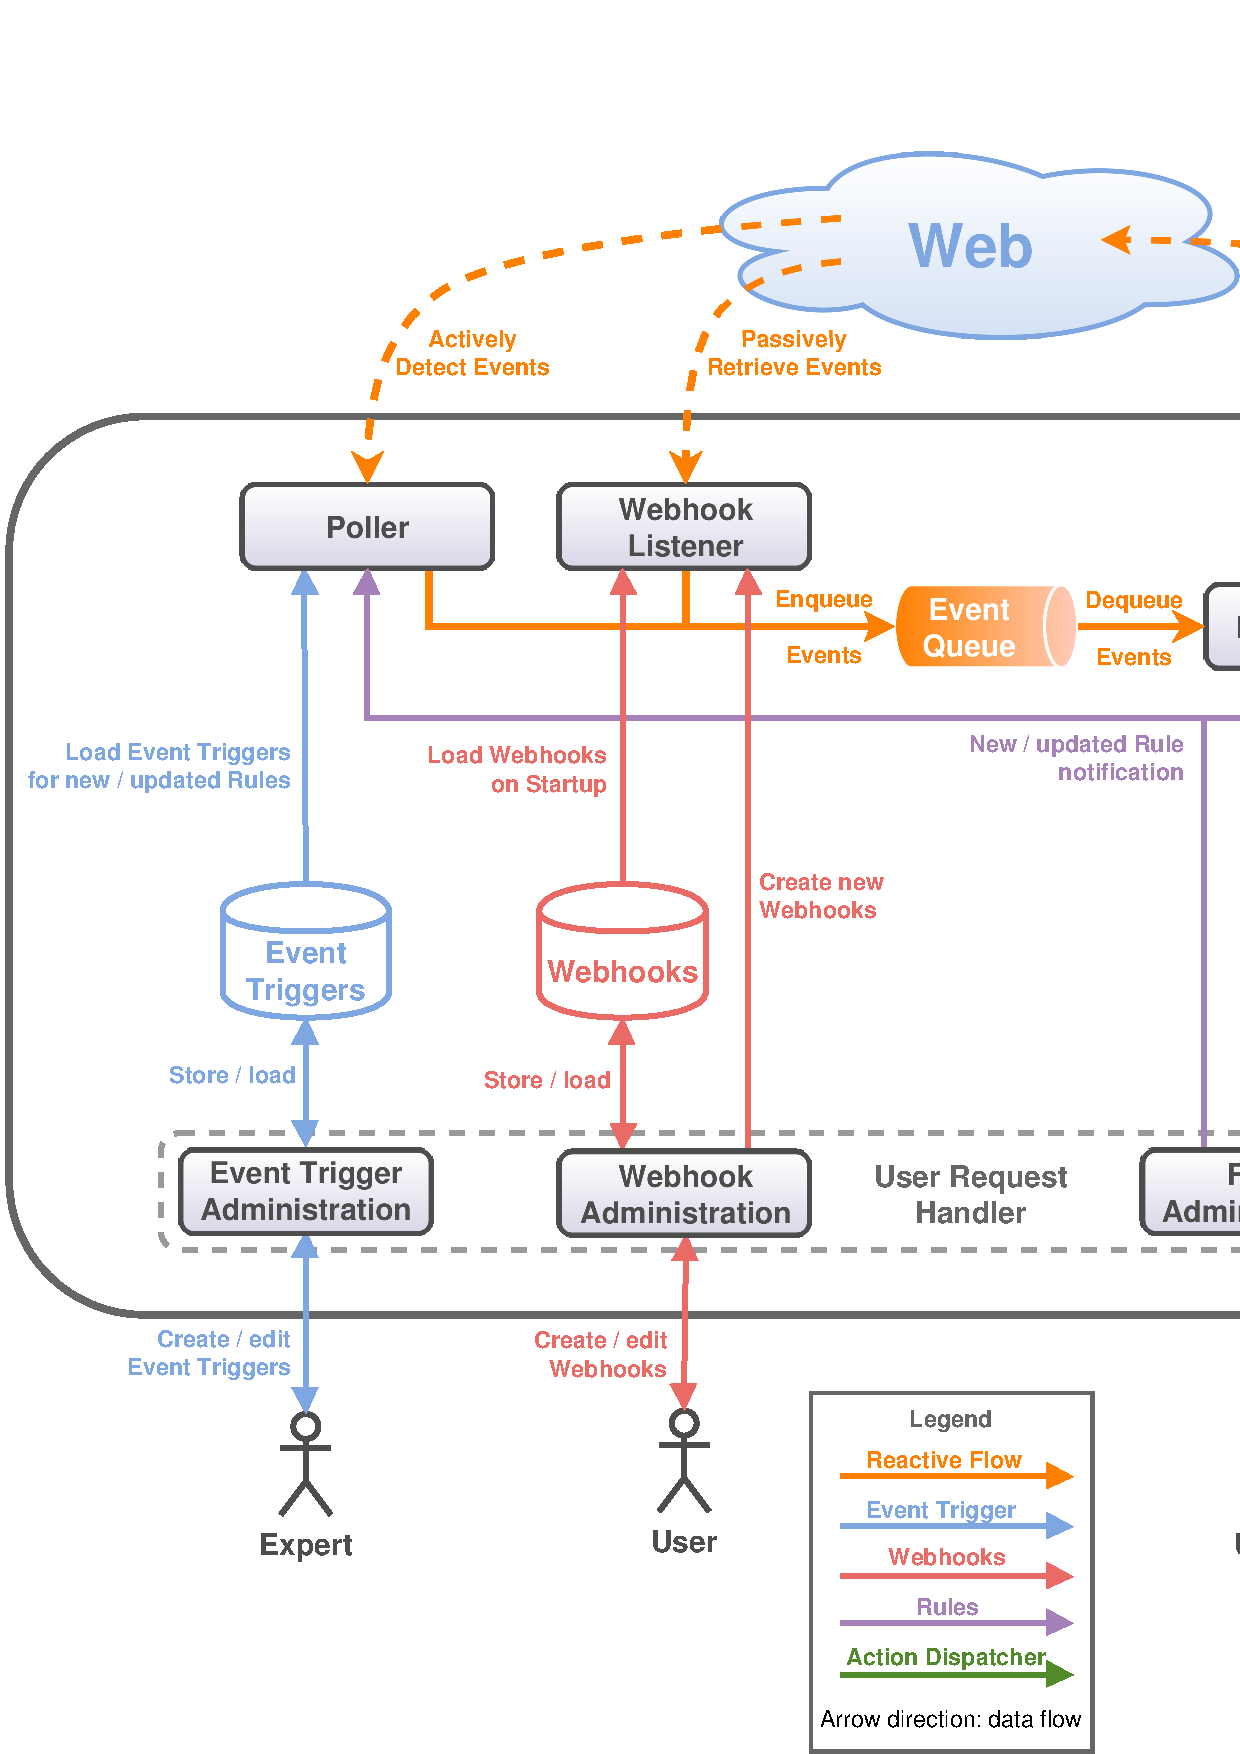
\includegraphics[width=\textwidth]{figures/Architecture_Final}
	\caption{Prototype System Architecture}
	\label{fig:Architecture}
\end{figure}



\subsection{Data Structure for Event Parameters}
Events in our prototype system are internally represented as tree structures in \textrm{\acrshort{json}} format.
The \textrm{\acrshort{json}} format builds on two data structures:
\begin{itemize}
	\item Objects: Unordered collections of name/value pairs wrapped in curly brackets \texttt{\{ \}}, which can also be implemented as a hash map, dictionary or struct in other languages.
	\item Arrays: Ordered lists of values wrapped in brackets \texttt{[ ]}, which can also be implemented as a record, vector or list in other languages.
\end{itemize}
A value can be an object or an array, but also a unicode string, a number, a boolean value or null.
This allows for any arbitrary depth and chaining of the supported data representations.
It is a handy feature when we assume a tree structure for events in our prototype system since the selection of nodes in tree structures has been well studied and useful libraries exist.
\textrm{\acrshort{json}} formatted datastructures can easily be marshaled into one string and communicated to other applications without overhead
Also, they are natively supported within \textrm{JavaScript} programming code. 
\textrm{\acrshort{json}} can be implemented in virtually every programming language, therefore received a lot of attention and is supported by many \textrm{\glspl{webresource}} for communication.



\subsection{Dynamic Code Loading for Event Trigger and Action Dispatcher}
During our research we have seen many different \textrm{\glspl{webservice}} with thoroughly different requirements in terms of communication.
The cleanest category among them were the \textrm{\glspl{webapi}} with their \textrm{\acrshort{rest}}ful services.
And still, in many cases it is only possible to access data which does not refer to an event.
To detect a change in data over time we need to be able to store an earlier request and get the difference to the current request, which could then be transformed into a meaningful event.
The derivation of a meaningful event from data can be a complex task which requires certain operations, which underlines the need for powerful \textrm{Event Trigger} modules.
The complexity is even bigger for \textrm{Action Dispatcher} modules which alter data and require more complex communication to \textrm{\glspl{webservice}}.
For those reasons we made the decision to keep these modules flexible in terms of communication.
We also wanted to leave it open to expert users to encapsulate complicated logic into them for inexperienced users.
We modeled the \textrm{Event Trigger} and \textrm{Action Dispatcher} to be \textrm{JavaScript} code modules, which are created by expert users during runtime.
They are also loaded during runtime whenever an activated rule needs them.
These modules run in a sandbox and got only access to certain \textrm{JavaScript} libraries, which are provided by the owner of the system.
Through this it is possible to communicate with \textrm{\acrshort{rest}}ful \textrm{\glspl{webservice}} as well as with \textrm{\acrshort{soap}} \textrm{\glspl{webService}} or any other service that can be addressed through \textrm{JavaScript} libraries. 
Apart from those libraries there are two other important functions offered in both type of modules:
\begin{itemize}
	\item \textrm{log}: Will store log entries on a per rule base, wherever the instruction is met during execution of a module.
	The log can be seen by the user who chose the module to be part of a rule.
	\item \textrm{pushEvent}: This funciton is an important part of \textrm{Event Trigger} modules.
	It is responsible to push events into the prototype system. For \textrm{Action Dispatcher} modules this provides the possibility for loopback events.
\end{itemize}
Only functions which are attached to the \texttt{exports} property of the module are later accessible from the outside and can be selected as \textrm{Event Trigger} or \textrm{Action Dispatcher}.
The function arguments of, from outside visible, functions are identified by the according \textrm{User Request Handler} module and the user will be requested to provide values for all of them in order to activate the \textrm{Event Trigger} or \textrm{Action Dispatcher}.
For \textrm{Action Dispatchers} it is also possible to use event property selectors as arguments and thus allows the passing of event data to the \textrm{Action Dispatchers}.
Through the \texttt{pushEvent} function in the global scope of the modules, events can be pushed into the prototype system.

By using the expressiveness of \textrm{JavaScript} and some of its libraries, it is possible to access a large part of the existing \textrm{\glspl{infosystem}} and transform changes in their \textrm{\glspl{infospace}} into events and also to impose changes onto them as part of actions.
The power that can be expressed in those code modules needs to be controlled, and ca not be granted to anybody, thus we shield it through user access control, thus only allowing trusted users to write \textrm{Event Trigger} and \textrm{Action Dispatcher} code.



\subsection{Retrieving Events}
In the last chapters, we put emphasis on the two different ways how events can be retrieved from \textrm{\glspl{infosystem}}, i.e. actively pulling events, or passively retrieving them.
Some \textrm{\glspl{infosystem}} offer access to data that corresponds to events and can instantly be forwarded into the system.
But we have seen that there is need for the derivation of events from changes in data on the Web, therefore we need the \textrm{Event Trigger} modules.
But still, our vision is that of an optimal real-time reactive Web which means that all possible events are offered by all \textrm{\glspl{infosystem}}.
An interested remote entity could announce interest in a certain kind of events over a \textrm{\gls{webhook}} and would retrieve them in real-time.
For that reason we laid out our architecture for \textrm{\glspl{webhook}}, but still offer the \textrm{Event Trigger} modules to poll for events in the semi-static \textrm{\gls{www}}.
During prototype testing we focused mainly on server-sided \textrm{Web APIs}, but we also generated events from the browser and pushed them to our prototype system.
This was achieved with a library included in a sample webpage that pushed events to a \textrm{\gls{webhook}} of our prototype.
Since modern browsers support geo locating, we decided to let the client browser push the current position of the device to the \textrm{\gls{webhook}}.



\subsubsection{Polling with Event Triggers}
As we have pointed out before, \textrm{Event Trigger} modules are dynamic code modules with access to a set of predefined libraries.
The \textrm{Poller} loads \textrm{Event Trigger} modules whenever they are required in an active rule.
The user of the \textrm{Event Trigger} can choose a starting point and an interval for the polling to take place.
An example \textrm{\gls{webservice}} which offers polling for events is the \textrm{Email Yak}\footnote{http://www.emailyak.com/} \textrm{\gls{webapi}}, which responds with new emails when requested.
The code required to request the new mails from this service and forward them into the prototype system is quite short and shown in Listing \ref{lst:emailyak}.
For other services it can quickly get more complex, depending on how complicated a meaningful change detection is.
For better readability the code is written in \textrm{CoffeeScript}\footnote{http://coffeescript.org/}.
Only expert users are expected to store such a piece of code in our prototype, which enables inexperienced users to simply choose the \texttt{"EmailYak -> newMail"} \textrm{Event Trigger} for their rule.  
A great opportunity to access data from webpages via a \textrm{\gls{webapi}} is \textrm{Import.io}\footnote{https://import.io/}.
By browsing through the Web with the \textrm{Import.io} browser, it is possible to select certain parts from a webpage and store the selection as a mask.
Data is instantly extracted from the webpage, using the stored mask, when sending a request to their \textrm{\gls{webapi}} with the given mask id and the \textrm{\acrshort{uri}}.
This is a great tool for expert users to predefine desired data on webpages and then produce events out of an \textrm{Event Trigger} whenever there is a change in that data.
\begin{lstlisting}[float=h,label=lst:emailyak,language=CoffeeScript,caption=Event Trigger code to poll Email Yak RESTful Web service for new Mails; written in CoffeeScript]
url = "https://api.emailyak.com/v1/#{params.apikey}/json/get/new/email/"
exports.newMail = () ->
	needle.get url, ( err, resp, body ) ->
		if not err and resp.statusCode is 200
				pushEvent mail for mail in body.Emails
\end{lstlisting}



\subsubsection{\gls{webhook}}
As powerful as their ability to provide real-time notifications from remote \textrm{\glspl{webresource}} is, as simple are \textrm{\glspl{webhook}} to use.
In our prototype, users can create as many new \textrm{\gls{webhook}} as they like.
They only need to provide an event name which will be associated to the \textrm{\gls{webhook}}.
A new \textrm{\gls{webhook}} is created in the \textrm{\gls{webhook} Listener}, which from then on accepts events posted to it.
The \textrm{\gls{webhook} \acrshort{uri}} is always accessible to the user and can be placed at any desired \textrm{\gls{webhook}} in order to receive events from it.
Any \textrm{\gls{webresource}} that supports the concept of \textrm{\gls{webhook}} (e.g. \textrm{GitHub}\footnote{https://developer.github.com/\gls{webhook}/}) has a place to register the \textrm{\gls{webhook}} \textrm{\acrshort{uri}}.
Whenever a remote \textrm{\gls{webresource}} pushes an event to the \textrm{\gls{webhook}}, the user-defined event name is assigned as the implicit parameter of a freshly created internal event.
The whole incoming event body is added as explicit parameters to the internal event, which is forwarded to the \textrm{Event Queue}.



\subsection{Dispatching Actions}
\textrm{Action Dispatchers} are \textrm{JavaScript} code modules that can be created during runtime and loaded by the engine whenever a new rule requires them, much as the \textrm{Event Trigger} modules are loaded by the \textrm{Poller}.
Before actions can be used in a rule, an expert has to create them.
In our prototype system, \textrm{Action Dispatchers} use a library for \textrm{HTTP} communication which allows them to address a wide range of \textrm{\glspl{webresource}}.
\textrm{Action Dispatchers} can also push events back into the \textrm{Event Queue} which can be used to chain certain rules together.
Since \textrm{\glspl{webhook}} are an important part of our vision we also implemented an \textrm{Action Dispatcher} that delivers events to external \textrm{\gls{webhook}}.
\textrm{Action Dispatchers} need to have functions attached to their \texttt{exports} property so that they are visible from the outside and can be selected as actions, such as the \texttt{newContent} function in the example Listing \ref{lst:actionProBinder}.
\begin{lstlisting}[float=h,label=lst:actionProBinder,language=CoffeeScript,caption=Action Dispatcher code to store a new content on the ProBinder RESTful Web service; written in CoffeeScript]
urlService = 'https://probinder.com/service/'

requestService = ( args ) ->
  url = urlService + args.service + '/' + args.method
  needle.post url, args.data

exports.newContent = ( companyId, contextId, content ) ->
  requestService
    service: 'content'
    method: 'save'
    data:
      companyId: companyId
      context: contextId
      text: content
\end{lstlisting}



\subsection{\acrshort{eca} Rules in the Rule Engine}
While a car engine converts potential energy into mechanical work, our \textrm{Rule Engine} converts events into changes in \textrm{\glspl{infosystem}}.
We have introduced \textrm{\acrshort{eca}} rules as sufficient approach to impose reactivity on systems and adopted the \textrm{\acrshort{eca}} paradigm for our conceptual model.
For our prototype this means that the \textrm{Rule Engine} requires user-defined \textrm{\acrshort{eca}} rules which are compared against incoming events.
The \textrm{Rules Administration} within the \textrm{User Request Handler} notifies the \textrm{Rules Engine} about new or updated rules from the user, which then in turn loads required \textrm{Action Dispatcher} modules.
For each event in the \textrm{Event Queue}, the engine checks it against its stored \textrm{\acrshort{eca}} rules and dispatches actions whenever the event conforms to the rule's condition part.
The three parts of an \textrm{\acrshort{eca}} rule have the following requirements in our prototype system:
\begin{itemize}
	\item Event name: Any arbitrary Unicode string, can refer to the name of an \textrm{Event Trigger} or a \textrm{\gls{webhook}}, but also to a custom loopback event.
	\item Conditions: Zero or more instructions to be evaluated against an event. Requires a selector for a node in the tree structure of the event, a comparison operator ($<$, $<=$, $>$, $>=$, $==$, $!=$ or $instr$) and a value.
	\item Action Dispatchers: A list of \textrm{Action Dispatchers} to be invoked if all conditions of the given event evaluate to true. We assume that invocations can be expressed using common function invocation syntax ( i.e. \texttt{actionFunction(param1, param2[, ...])} ) in order to dispatch an action.
\end{itemize}
A valid rule in the internal \textrm{\acrshort{json}} representation is shown in Listing \ref{lst:rulejson}, where we used the predefined \textrm{EmailYak Action Dispatcher} to send a mail to an interested person whenever news about soccer are detected.

\subsubsection{Parameter Selectors for Events}
Tree node selectors for event parameters are used in conditions to select a parameter which is evaluated.
The selectors can also be used to pass event parameters as arguments to the \textrm{Action Dispatchers}.
Event tree node selectors for \textrm{Action Dispatcher} arguments are defined by wrapping them into curly brackets and prepended with a hash: \texttt{"\#\{ [selector] \}"}.
Since an existing \textrm{JavaScript} library\footnote{https://github.com/harthur/js-select} is used to find event parameters with selectors, the following selectors are available\footnote{Explanations taken from http://jsonselect.org/, which is used by js-select}:
\begin{itemize}
	\item \textrm{\textbf{* :}}	Any node
	\item \textrm{\textbf{T :}}	A node of type T, where T is one string, number, object, array, boolean, or null
	\item \textrm{\textbf{T.key :}}	A node of type T which is the child of an object and is the value its parents key property
	\item \textrm{\textbf{T:root :}}	A node of type T which is the root of the JSON document
	\item \textrm{\textbf{T:nth-child(n) :}}	A node of type T which is the nth child of an array parent
	\item \textrm{\textbf{T:nth-last-child(n) :}}	A node of type T which is the nth child of an array parent counting from the end
	\item \textrm{\textbf{T:first-child :}}	A node of type T which is the first child of an array parent (equivalent to T:nth-child(1)
	\item \textrm{\textbf{T:last-child :}}	A node of type T which is the last child of an array parent (equivalent to T:nth-last-child(1)
	\item \textrm{\textbf{T:only-child :}}	A node of type T which is the only child of an array parent
	\item \textrm{\textbf{T U :}}	A node of type U with an ancestor of type T
	\item \textrm{\textbf{T $>$ U :}}	A node of type U with a parent of type T
	\item \textrm{\textbf{T $\sim$ U :}}	A node of type U with a sibling of type T
	\item \textrm{\textbf{S1, S2 :}}	Any node which matches either selector S1 or S2
	\item \textrm{\textbf{T:has(S) :}}	A node of type T which has a child node satisfying the selector S
	\item \textrm{\textbf{T:val(V) :}}	A node of type T with a value that is equal to V
	\item \textrm{\textbf{T:contains(S) :}}	A node of type T with a string value contains the substring
\end{itemize}
\begin{Verbatim}[samepage=true,frame=single,fontsize=\footnotesize,commandchars=\\\{\},numbers=left,firstnumber=1,stepnumber=1,xleftmargin
=.3in]
\PY{p}{\PYZob{}}
  \PY{n+nt}{\PYZdq{}eventname\PYZdq{}}\PY{p}{:} \PY{l+s+s2}{\PYZdq{}news\PYZdq{}}\PY{p}{,}
  \PY{n+nt}{\PYZdq{}conditions\PYZdq{}}\PY{p}{:} \PY{p}{[}
    \PY{p}{\PYZob{}}
      \PY{n+nt}{\PYZdq{}selector\PYZdq{}}\PY{p}{:} \PY{l+s+s2}{\PYZdq{}.categories\PYZdq{}}\PY{p}{,}
      \PY{n+nt}{\PYZdq{}operator\PYZdq{}}\PY{p}{:} \PY{l+s+s2}{\PYZdq{}instr\PYZdq{}}\PY{p}{,}
      \PY{n+nt}{\PYZdq{}compare\PYZdq{}}\PY{p}{:} \PY{l+s+s2}{\PYZdq{}soccer\PYZdq{}}
    \PY{p}{\PYZcb{}}
  \PY{p}{]}\PY{p}{,}
  \PY{n+nt}{\PYZdq{}actions\PYZdq{}}\PY{p}{:}\PY{p}{[}
    \PY{l+s+s2}{\PYZdq{}EmailYak\PYZhy{}\PYZgt{}sendMail(\PYZbs{}\PYZdq{}fan@soccer.com\PYZbs{}\PYZdq{},\PYZbs{}\PYZdq{}News about soccer!\PYZbs{}\PYZdq{},\PYZbs{}\PYZdq{}\PYZsh{}\PYZob{} .body \PYZcb{}\PYZbs{}\PYZdq{})\PYZdq{}}
  \PY{p}{]}
\PY{p}{\PYZcb{}}
\end{Verbatim}
\vspace{-0.7cm}
\begin{lstlisting}[float=h,frame=no,label=lst:rulejson,caption=Rule Example expressed in \textrm{\acrshort{json}}]
\end{lstlisting}

\section{A Rule Language for the Prototype System}
So far, we introduced the internal representation of the \textrm{\acrshort{eca}} rule language used in our prototype system.
For human readability and more intuitive writing, they can be transformed into a phrase representation, through which Listing \ref{lst:rulejson} would be written as shown in Listing \ref{lst:exampleRulePhrase}.
Our language is descriptive and flexible in terms of the \textrm{Event Trigger} and \textrm{Action Dispatcher} modules.
Another important flexible factor is the mapping of event properties to the \textrm{Action Dispatchers}.
To write a rule it requires a priori information from the \textrm{Event Trigger} and \textrm{Action Dispatcher} modules, but we believe this can be offered intuitively to the user through today's \textrm{\glspl{webapplication}}.
Listing \ref{lst:exampleRulePhrase} shows an example phrase of our envisioned rule language where the retrieval of a new mail will be checked for soccer news and, if confirmed, the mail body will be forwarded to an interested person.
The Extended Backus-Naur Form for the prototype rule language syntax is shown in Listing \ref{lst:backusnaur}.

\begin{lstlisting}[float=h,language=OwnRule,label={lst:exampleRulePhrase},caption=Example Phrase in Prototype Rule Language]
ON news
IF ".categories" instr "soccer"
DO EmailYak->sendMail("fan@soccer.com","News about soccer!","#{ .body }")
\end{lstlisting}

\begin{lstlisting}[float=h,language=OwnRule,label={lst:backusnaur},caption={Extended Backus-Naur Form of Prototype Rule Language Syntax}]
expression  ::= "ON " event " IF " conditions " DO " actions
event       ::= word* ("->" word+)?
conditions  ::= condition (" AND " condition)*
condition   ::= string operator "'" string "'"
operator    ::= (" < "|" <= "|" > "|" >= "|" == "|" != "|" instr ")
actions     ::= action (", " action)*
action      ::= word* "(" (argument ("," argument)*)? ")"
argument    ::= "'" selstring "'"
selstring   ::= (word|selector|" ")
selector    ::= "#{" string "}"
string      ::= (word|special|" ")*
special     ::= [():.*>~,]
word        ::= [A-Za-z0-9_-]+
\end{lstlisting}



\section{Prototype Use Case Implementations}
In the previous chapter we listed use cases for our conceptual model.
In this chapter we introduce use cases that were implemented in our prototype system in order to impose reactivity on the \textrm{\gls{web}}.


\subsection{Detecting responding Computers}
In our department building, one office is located on the other side of the floor and the elevator is right in the middle of it.
This resulted in one person frequently missing the coffee break, because everybody was always in a lively discussion towards the elevator and forgot about him.
Thus he sat up a network scanner that pinged the department's \textrm{Internet Protocol (IP)} range in the morning and pushed the results as events into the system.
Through this he was able to set up a rule that, if more than 42 pings were returned, the system automatically deployed an email invitation to the group, suggesting a coffee break.
The network scanner (code in Appendix \ref{lst:eventproducer}) was implemented as external \textrm{\gls{infosystem}} which pushed the ping results as event over a \textrm{\gls{webhook}}.
The rule is shown in Listing \ref{lst:ruleCoffeeBreak} and the corresponding simplified \textrm{Action Dispatcher} is shown in Listing \ref{lst:adEmailYak}.

\begin{Verbatim}[samepage=true,frame=single,fontsize=\footnotesize,commandchars=\\\{\},numbers=left,firstnumber=1,stepnumber=1,xleftmargin
=.3in]
\PY{p}{\PYZob{}}
  \PY{n+nt}{\PYZdq{}eventname\PYZdq{}}\PY{p}{:} \PY{l+s+s2}{\PYZdq{}uptimestatistics\PYZdq{}}\PY{p}{,}
  \PY{n+nt}{\PYZdq{}conditions\PYZdq{}}\PY{p}{:} \PY{p}{[}
    \PY{p}{\PYZob{}}
      \PY{n+nt}{\PYZdq{}selector\PYZdq{}}\PY{p}{:} \PY{l+s+s2}{\PYZdq{}.currentlyon\PYZdq{}}\PY{p}{,}
      \PY{n+nt}{\PYZdq{}operator\PYZdq{}}\PY{p}{:} \PY{l+s+s2}{\PYZdq{}\PYZgt{}\PYZdq{}}\PY{p}{,}
      \PY{n+nt}{\PYZdq{}compare\PYZdq{}}\PY{p}{:} \PY{l+m+mi}{42}
    \PY{p}{\PYZcb{}}
  \PY{p}{]}\PY{p}{,}
  \PY{n+nt}{\PYZdq{}actions\PYZdq{}}\PY{p}{:} \PY{p}{[}
    \PY{l+s+s2}{\PYZdq{}EMailYak \PYZhy{}\PYZgt{} sendMail(\PYZbs{}\PYZdq{}eca\PYZhy{}engine@mscliveweb.simpleyak.com\PYZbs{}\PYZdq{},[usermaillist],}
\PY{l+s+s2}{      \PYZbs{}\PYZdq{}Coffee Break!\PYZbs{}\PYZdq{},\PYZbs{}\PYZdq{}Let\PYZsq{}s go for a coffee at 10!\PYZbs{}\PYZdq{})\PYZdq{}}
  \PY{p}{]}
\PY{p}{\PYZcb{}}
\end{Verbatim}
\vspace{-0.7cm}
\begin{lstlisting}[float=h,language=OwnRule,caption={Rule; Coffee Break Invitation},label={lst:ruleCoffeeBreak},frame=no]
\end{lstlisting}

\begin{lstlisting}[float=h,language=CoffeeScript,caption={Action Dispatcher; EMailYak, in CoffeeScript},label={lst:adEmailYak}]
url = 'https://api.emailyak.com/v1/'+params.apikey+'/json/send/email/'

exports.sendMail = ( sender, receipient, subject, content ) ->
	data =
		FromAddress: sender
		ToAddress: receipient
		Subject: subject
		TextBody: content
	needle.post url, data, json: true
\end{lstlisting}


\subsection{Webpage Diff}




\subsection{Enhance Existing Web App}

\begin{lstlisting}[float=h,language=OwnRule,label={lst:RulePhraseAnnotate},caption=Rule Phrase for ProBinder Annotations]
ON ProBinder->unreadContent
IF "#{ .context .id }" == 18749
DO ProBinder->annotateTagEntries("#{ .id }"),
	 ProBinder->setRead("#{ .id }")
\end{lstlisting}


% on ProBinder->unreadContent
% if "#{ .context .id }" == 18749
% do "ProBinder -> annotateTagEntries(\"#{ .id }\")",
% 	 "ProBinder -> setRead(\"#{ .id }\")"
   

\subsection{Real-time Reactive Messenger}





% During our research we found a troublesome server room that made us develop a rule towards exposition of the \textrm{\gls{webofthings}}.
% This server room suffered from a defective cooling system which lead to a drastic increase of temperature in certain circumstances.
% As a consequence certain server automatically shut themselves down as safety measurements.
% In order to support the administrator we sat up 
% As a very quick fix to inform certain administrators about the shutdown of their server, we started pinging these servers and pushed the results int

\subsection{Page Rank of Webpage changes}


% Real-time reactive Web over \gls{webhook} -> instant messaging


% {
%     "dominic": {
%         "SOAP test": "{\"id\":\"SOAP test\",\"eventtype\":\"Custom Event\",\"eventname\":\"button-click\",\"conditions\":[],\"actions\":[\"SOAP -> convertCelsiusToFahrenheit\"]}",
%         "Presentation to Pushover": "{\"id\":\"Presentation to Pushover\",\"eventtype\":\"Custom Event\",\"eventname\":\"pushover\",\"conditions\":[],\"actions\":[\"Pushover -> broadcast\"]}",
%         "ProBinder Service Test: FAIL": "{\"id\":\"ProBinder Service Test: FAIL\",\"eventtype\":\"Custom Event\",\"eventname\":\"ProBinderServiceTest\",\"conditions\":[{\"selector\":\".success\",\"type\":\"bool\",\"operator\":\"==\",\"compare\":false}],\"actions\":[\"Pushover -> broadcast\",\"EMailYak -> sendMail\"]}",
%         "ProBinder Service Test": "{\"id\":\"ProBinder Service Test\",\"eventtype\":\"Event Poller\",\"eventname\":\"ProBinder Service Test -> testProBinder\",\"eventstart\":\"2014-05-20T13:00:00.000Z\",\"eventinterval\":120,\"conditions\":[],\"actions\":[\"System -> pushEvent\"],\"timestamp\":\"2014-05-20T11:51:46.307Z\"}",
%         "'button-click' Rule": "{\"id\":\"'button-click' Rule\",\"eventtype\":\"Custom Event\",\"eventname\":\"button-click\",\"conditions\":[],\"actions\":[\"Pushover -> broadcast\"]}",
%         "ProBinder annotate tags": "{\"id\":\"ProBinder annotate tags\",\"eventtype\":\"Event Poller\",\"eventname\":\"ProBinder -> unreadContent\",\"eventstart\":\"2014-05-20T19:11:00.000Z\",\"eventinterval\":1,\"conditions\":[],\"actions\":[\"ProBinder -> annotateTagEntries\",\"ProBinder -> setRead\"],\"timestamp\":\"2014-05-20T19:10:10.951Z\"}",
%         "Coffee Break": "{\"id\":\"Coffee Break\",\"eventtype\":\"Custom Event\",\"eventname\":\"uptimestatistics\",\"conditions\":[{\"selector\":\".currentlyon\",\"type\":\"value\",\"operator\":\">\",\"compare\":42}],\"actions\":[\"EMailYak -> sendMail\"]}",
%         "ProBinder Service Test: Logging": "{\"id\":\"ProBinder Service Test: Logging\",\"eventtype\":\"Custom Event\",\"eventname\":\"ProBinderServiceTest\",\"conditions\":[],\"actions\":[\"ProBinder -> newContent\"]}"
%     }
% }

\begin{figure}[!ht]
	\centering
  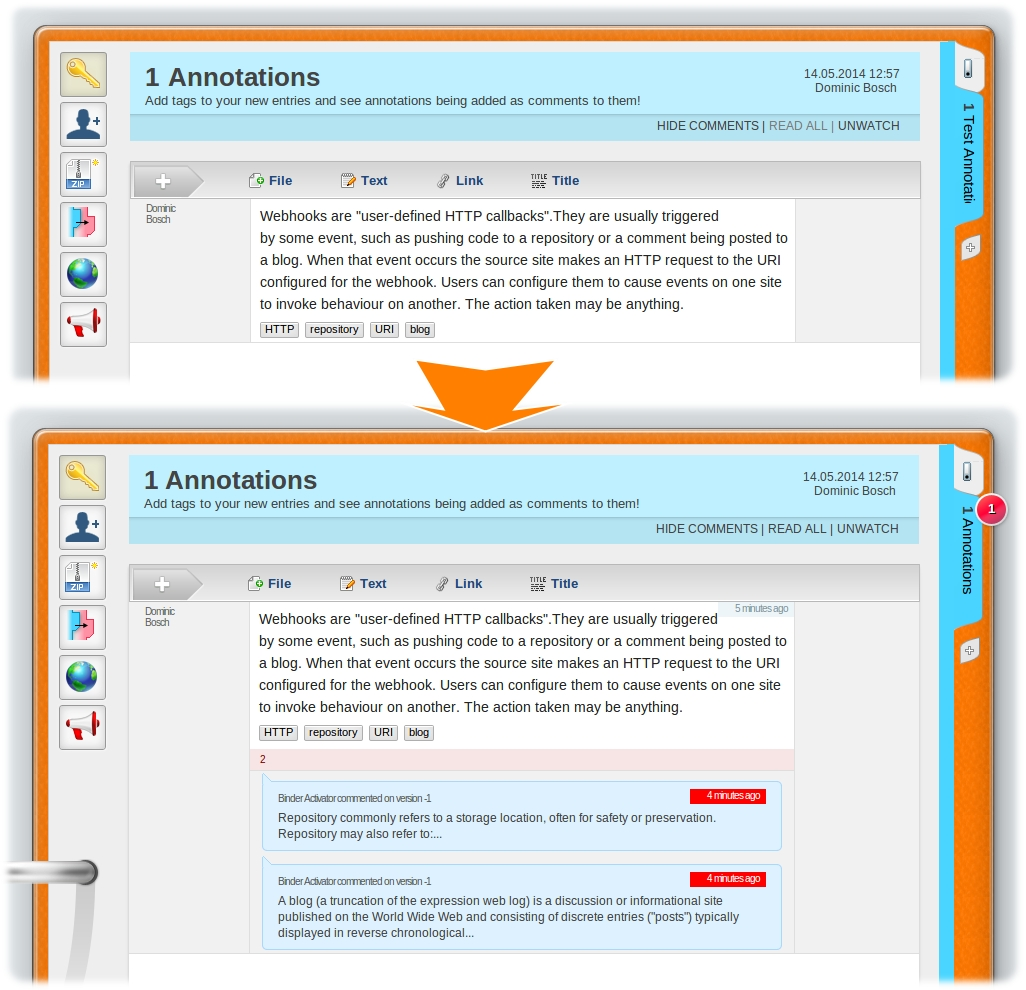
\includegraphics[width=\textwidth]{figures/UC_Binder_Annotations}
	\caption{UC Binder Annotation}
	\label{fig:UC_Binder_Annotations}
\end{figure}

\section{Web Application Development}
% Why JS, why was not it used up to now? is it used now?

% My guess is that Node is encouraging good programmer practices in terms of scalability, and Java less so. In other words, programmers probably have to work less hard to avoid bad scalability bottlenecks in Node than in Java.

% By incorporating JavaScript’s asynchronous design
% of callback functions into their architecture, locking situations are basically
% omitted. Thus it is a highly-scalable, asynchronous, event-driven architec-
% ture which found its acceptance in the open-source comunity as well as for
% enterprises.
% The package manager npm can be used to maintain dependencies of a
% custom node.js module to other modules. This helpful feature ensures that
% everybody working with the user-defined module uses the same external
% modules and the respective versions. Also project repositories do not need
% to store the dependent libraries through this mechanism, thus saving space


% full stack development 


% TODO why JS. JSON as first advantage (http://www.toptal.com/nodejs/why-the-hell-would-i-use-node-js)
% advantage for network applications with several concurrent connections
% not as client-server used as intented but as serverserver com since we also expect several connections simultanously under load.
% But also, we adopt the non-blocking nature of JS that is used for node's optimal communication, in order to implement our enigne in a non blocking way, thus allowing to load code and fire callback function in modules whenever they are required!
% http://ariya.ofilabs.com/2012/07/lazy-parsing-in-javascript-engines.html
% Optimization of special case if ( before function {immediately-invoked function expression (IIFE)}, do rela parsing, else lazy parsing
% Difference between context and scope. scope unique to each invocation, context is 'this', owner of currently executing code.
% .call, .apply 
% TODO we should use .bind for persistence.coffee's functions ....

%In JavaScript, functions are first-class objects, i.e. they are objects and can be manipulated and passed around just like any other object. Specifically, they are Function objects. -> https://developer.mozilla.org/en/docs/Web/JavaScript/Reference/Functions_and_function_scope
% Since each call provides potentially different arguments, a new closure is created for each call to outside. The memory can be freed only when the returned inside is no longer accessible

% The definitive guide: This combination of a function object and a scope (a set of variable bindings) in which the function’s variables are resolved is called a closure in the computer science literature.4
% This is an old term that refers to the fact that the function’s variables have bindings in the scope chain and that therefore the function is “closed over” its variables.



% Umgang mit der Zukunft
% Callback
\subsection{Callback Functions \& Asynchronous Closures}
% JAva futures? objekte für resultate sammeln
% Closures are functions that refer to independent (free) variables. 

Often, optimization approaches and programming language concepts require special attention to avoid common pitfalls.
When closures are used as asynchronous functions, developers need to be very careful not to end up with race conditions.


Looking at an example of sequential code execution in Figure~\ref{fig:Closures_Synchronous}, we see that function execution of \texttt{fA} is halted until function \texttt{fB} is finished.
If \texttt{fB} happens to be a latency-driven I/O operation the completion of \texttt{fA} could be deferred for a relatively long time.
While the application waits for the completion of the I/O operation, some remaining operations in \texttt{fA} could eventually already be executed without causing any race conditions.
\begin{figure}[!ht]
	\centering
  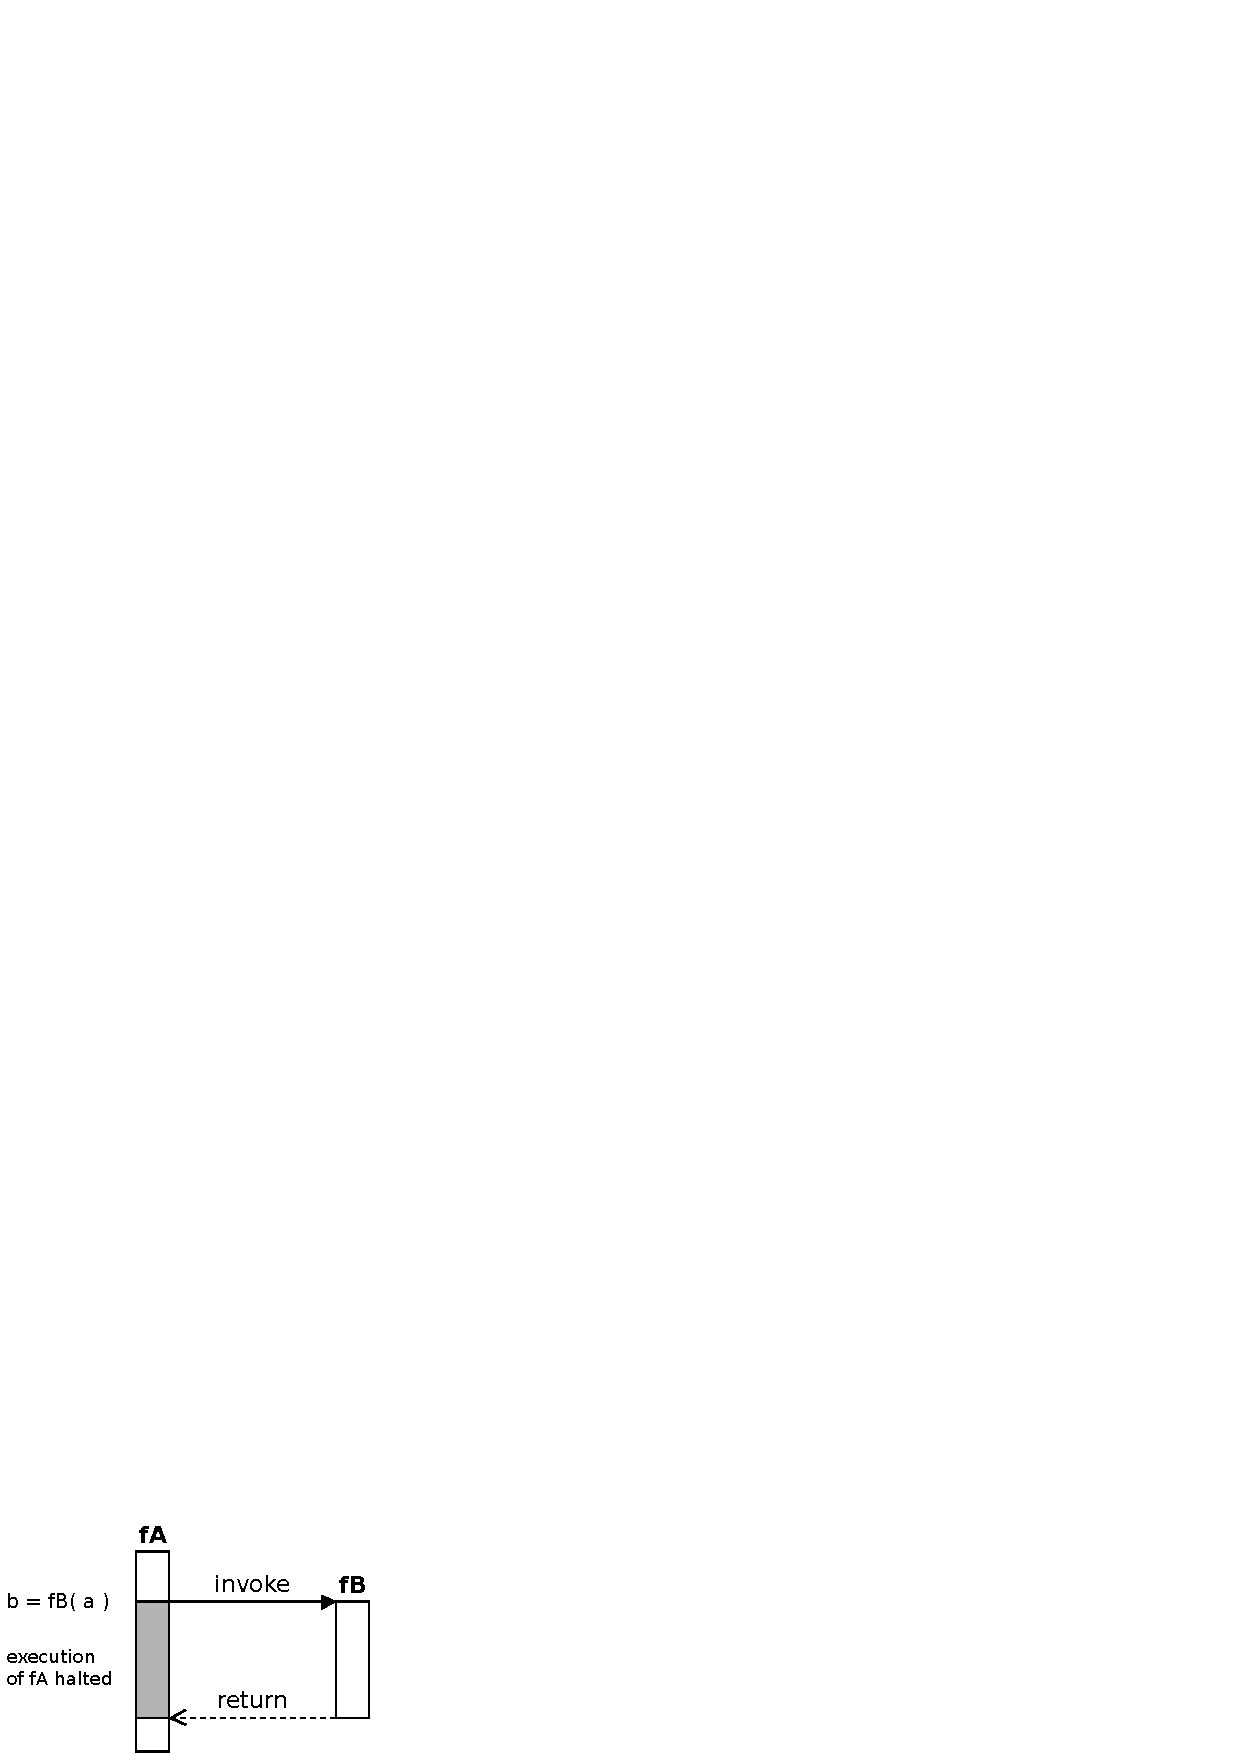
\includegraphics{figures/Closures_Synchronous}
	\caption{Synchronous Function Call}
	\label{fig:Closures_Synchronous}
\end{figure}

Asynchronous code execution, as shown in Figure~\ref{fig:Closures_Asynchronous}, allows non-blocking and thus scalable applications.
Non-blocking operations are a remedy for optimized resource allocation and open up ways to overcome previously described unnecessary resource bindings.
Processing any kind of latency-driven I/O operation asynchronously ( e.g. filesystem access and socket communication ) exploits resources that would otherwise be bound while waiting for completion.
Such operations are processed and completed whenever required resources are available.
\begin{figure}[!ht]
	\centering
  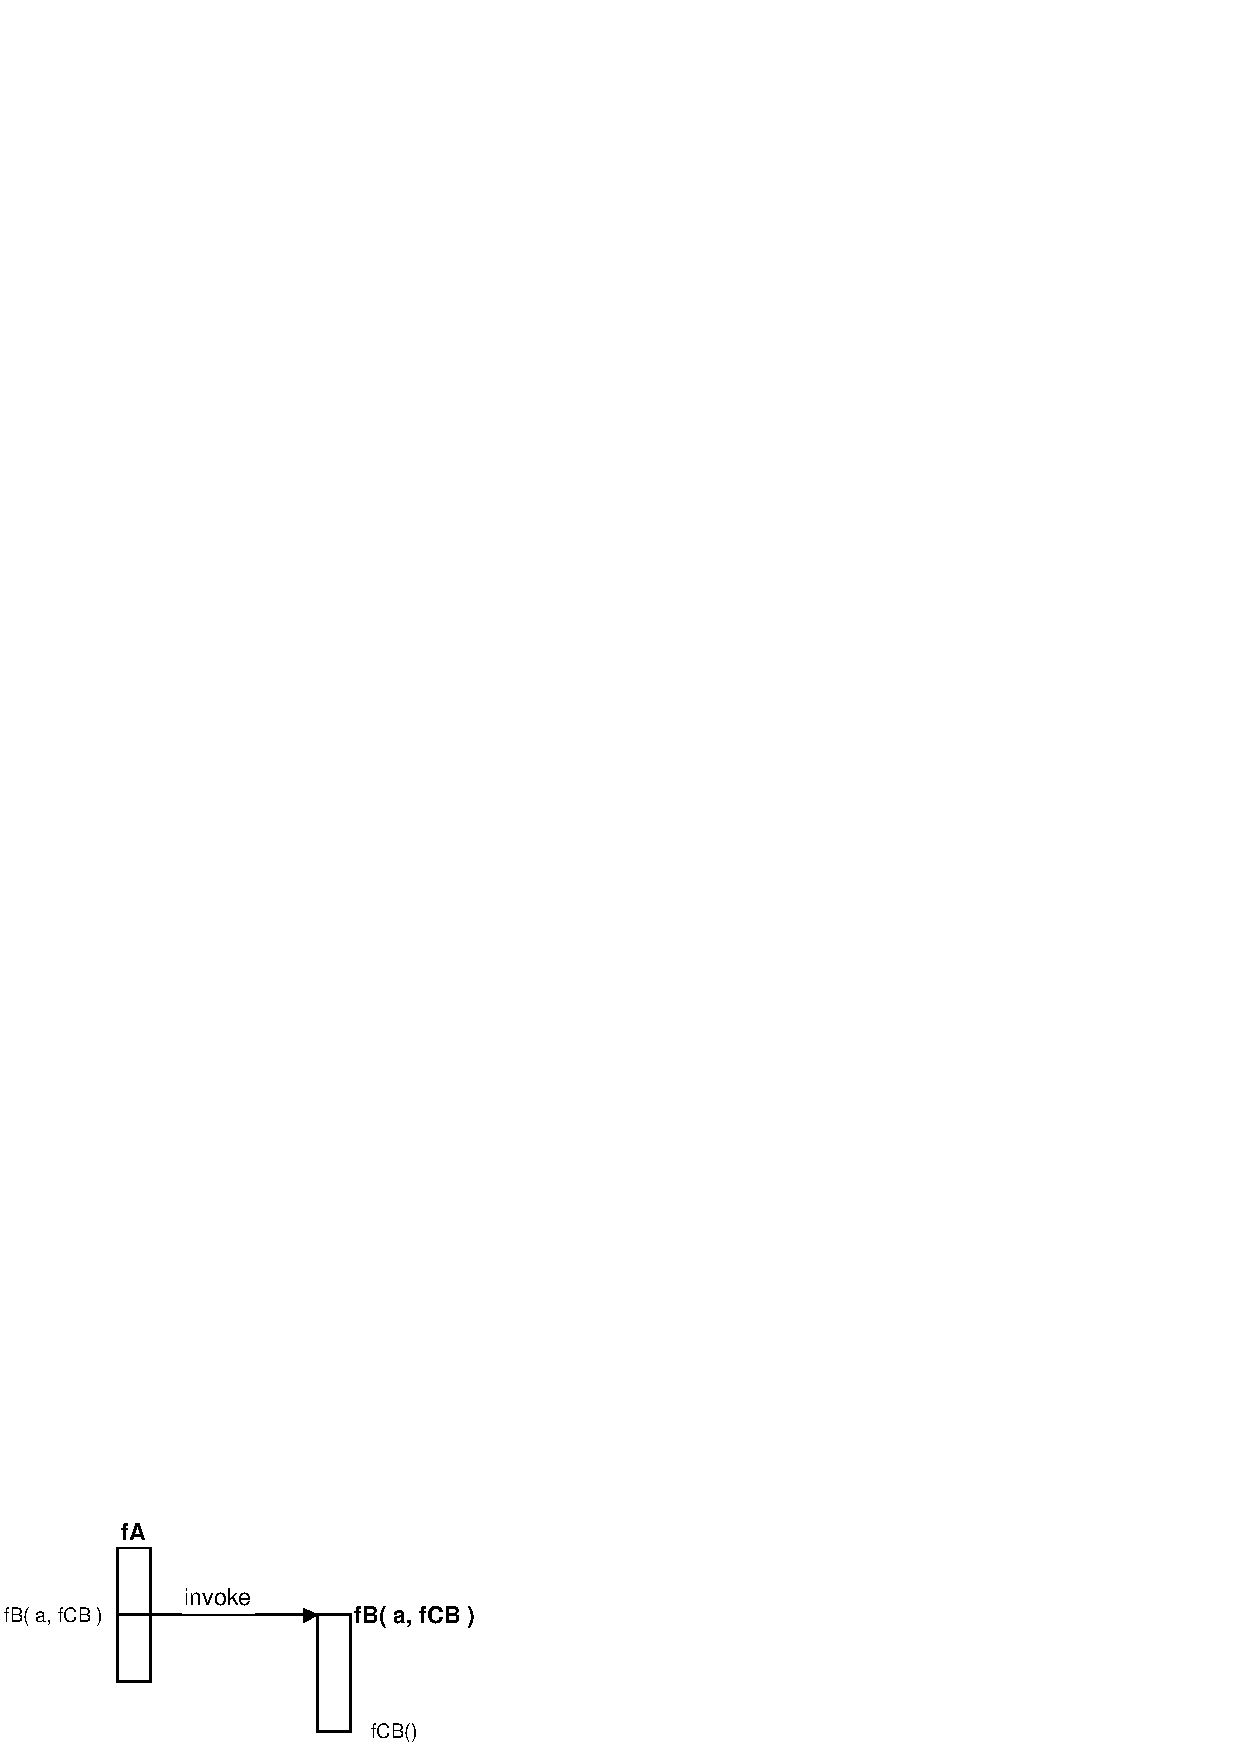
\includegraphics{figures/Closures_Asynchronous}
	\caption{Asynchronous Function Call}
	\label{fig:Closures_Asynchronous}
\end{figure}

Often other operations depend on the completion of asynchronous operations, hence their execution needs to be deferred.
This necessary code execution deferral is achieved through the use of callback functions, denoted \texttt{fCB} in Figure~\ref{fig:Closures_Asynchronous}.
Any code placed in a callback function, which is assigned to an asynchronous operation, is only executed after the respective asynchronous operation completed.
% TODO figure: Callback; Result ensurance (ergebnissichherung) wird direkt mit funktion mitgeschickt
This allows stacking of functions and operations upon each other which automatically results in a flexible and event-driven application.

So far we did not regard the context for such asynchronous functions.
If a function has access to the enclosing context where it was invoked in, it is called a closure.
Closures play an important role in \textrm{ECMAScript}\cite{EcmaScript}, which is the base for widely-spread script languages like JavaScript, JScript and ActionScript.
Closures in \textrm{ECMAScript} are defined such as they have access to the context of the function they were created in.
This is shown in Figure~\ref{fig:Closures_Closure-1} where \texttt{c} from \texttt{fA}'s context is accessible from within \texttt{fB}, assuming that \texttt{fB} was created in \texttt{fA} and not only invoked from there.
Closures make it necessary for the context of the outer function to survive past its execution so no references are broken.
This is labeled "extended context lifetime" in Figure~\ref{fig:Closures_Closure-1}.
Using asynchronous closures it becomes evident, that the context in the invoking function can change while the closure is still computing and eventually referencing the outer context, thus causing race conditions.
This will be most obvious in a loop that immediately invokes \texttt{fB} several times, as shown in Figure~\ref{fig:Closures_Closure-2}.
In such a setup \texttt{c} will have different values in the same part of different invocations of \texttt{fB}.
\begin{figure}[!ht]
	\centering
  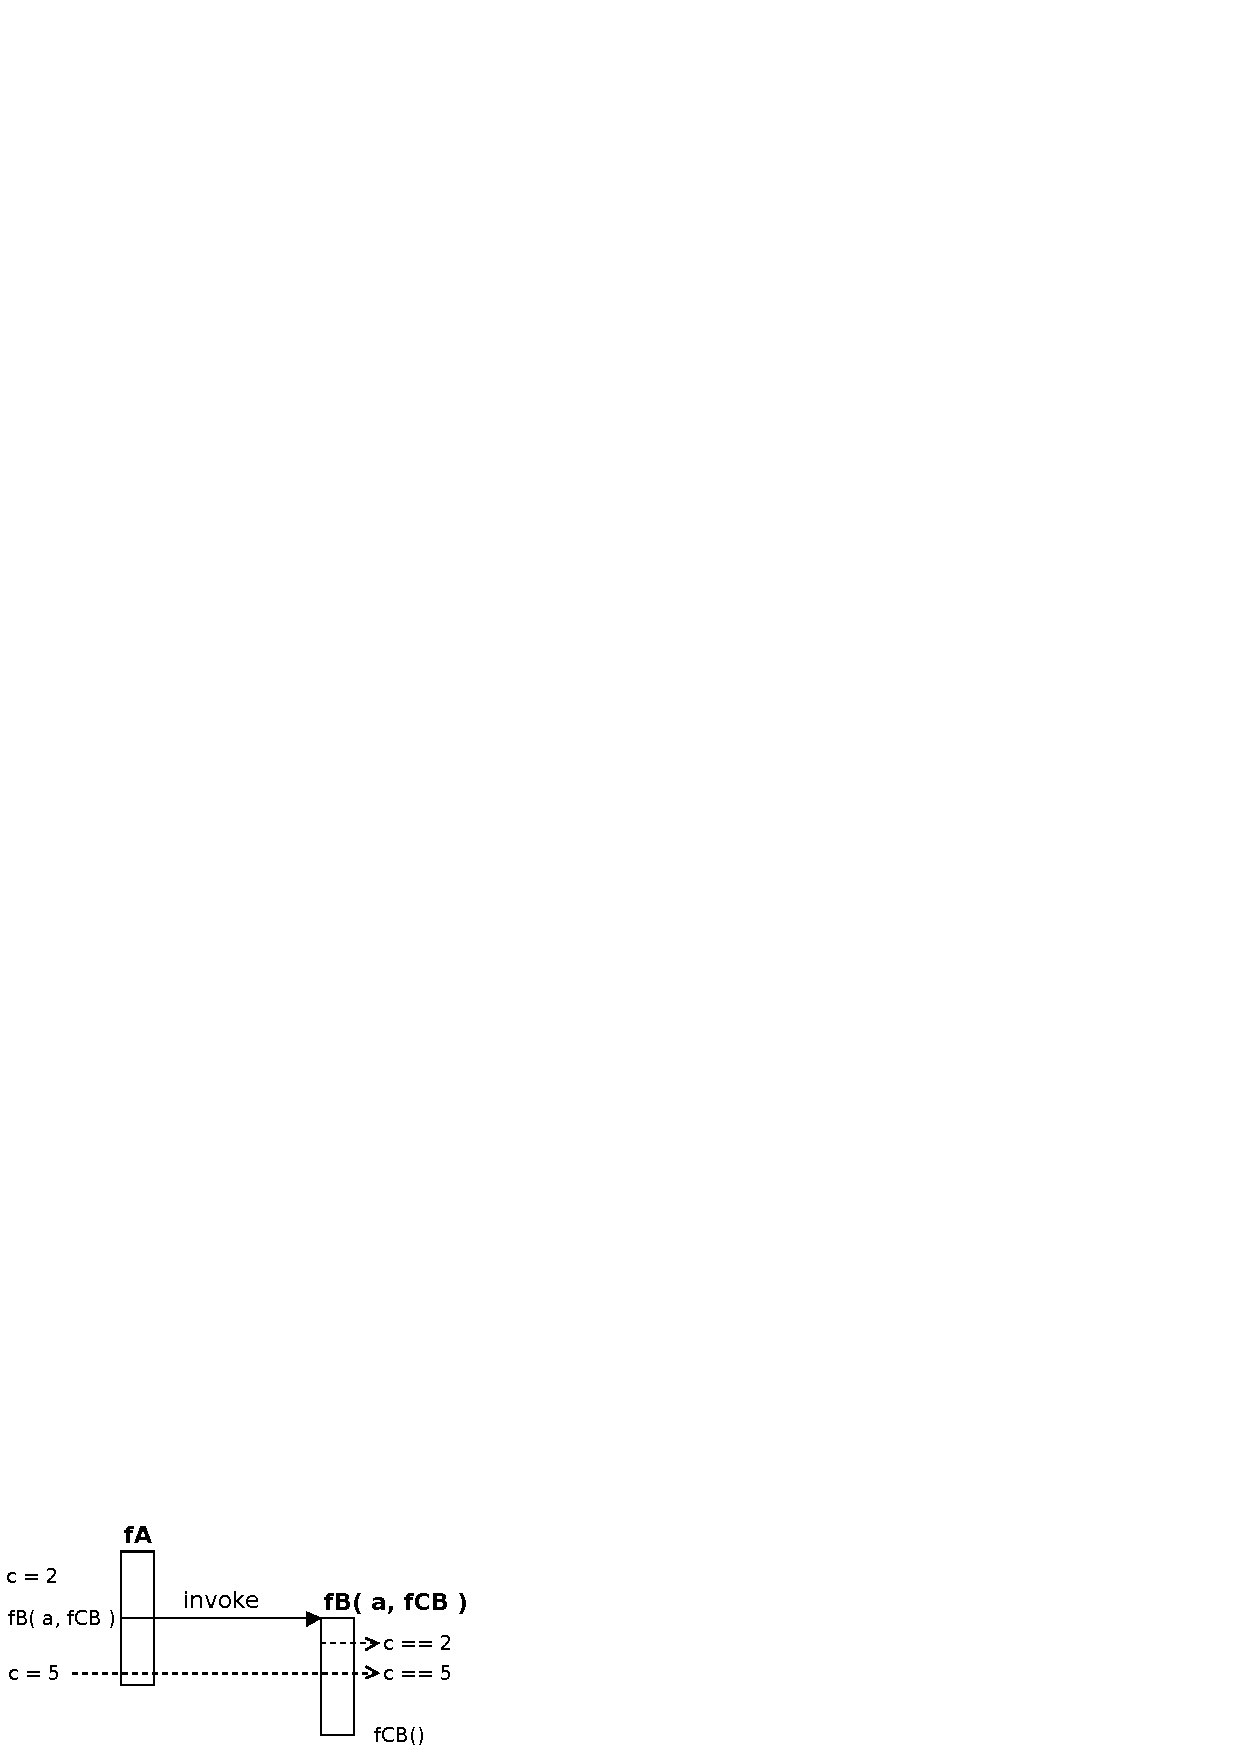
\includegraphics{figures/Closures_Closure-1}
	\caption{Closure Scope and referenced context}
	\label{fig:Closures_Closure-1}
\end{figure}
\begin{figure}[!ht]
	\centering
  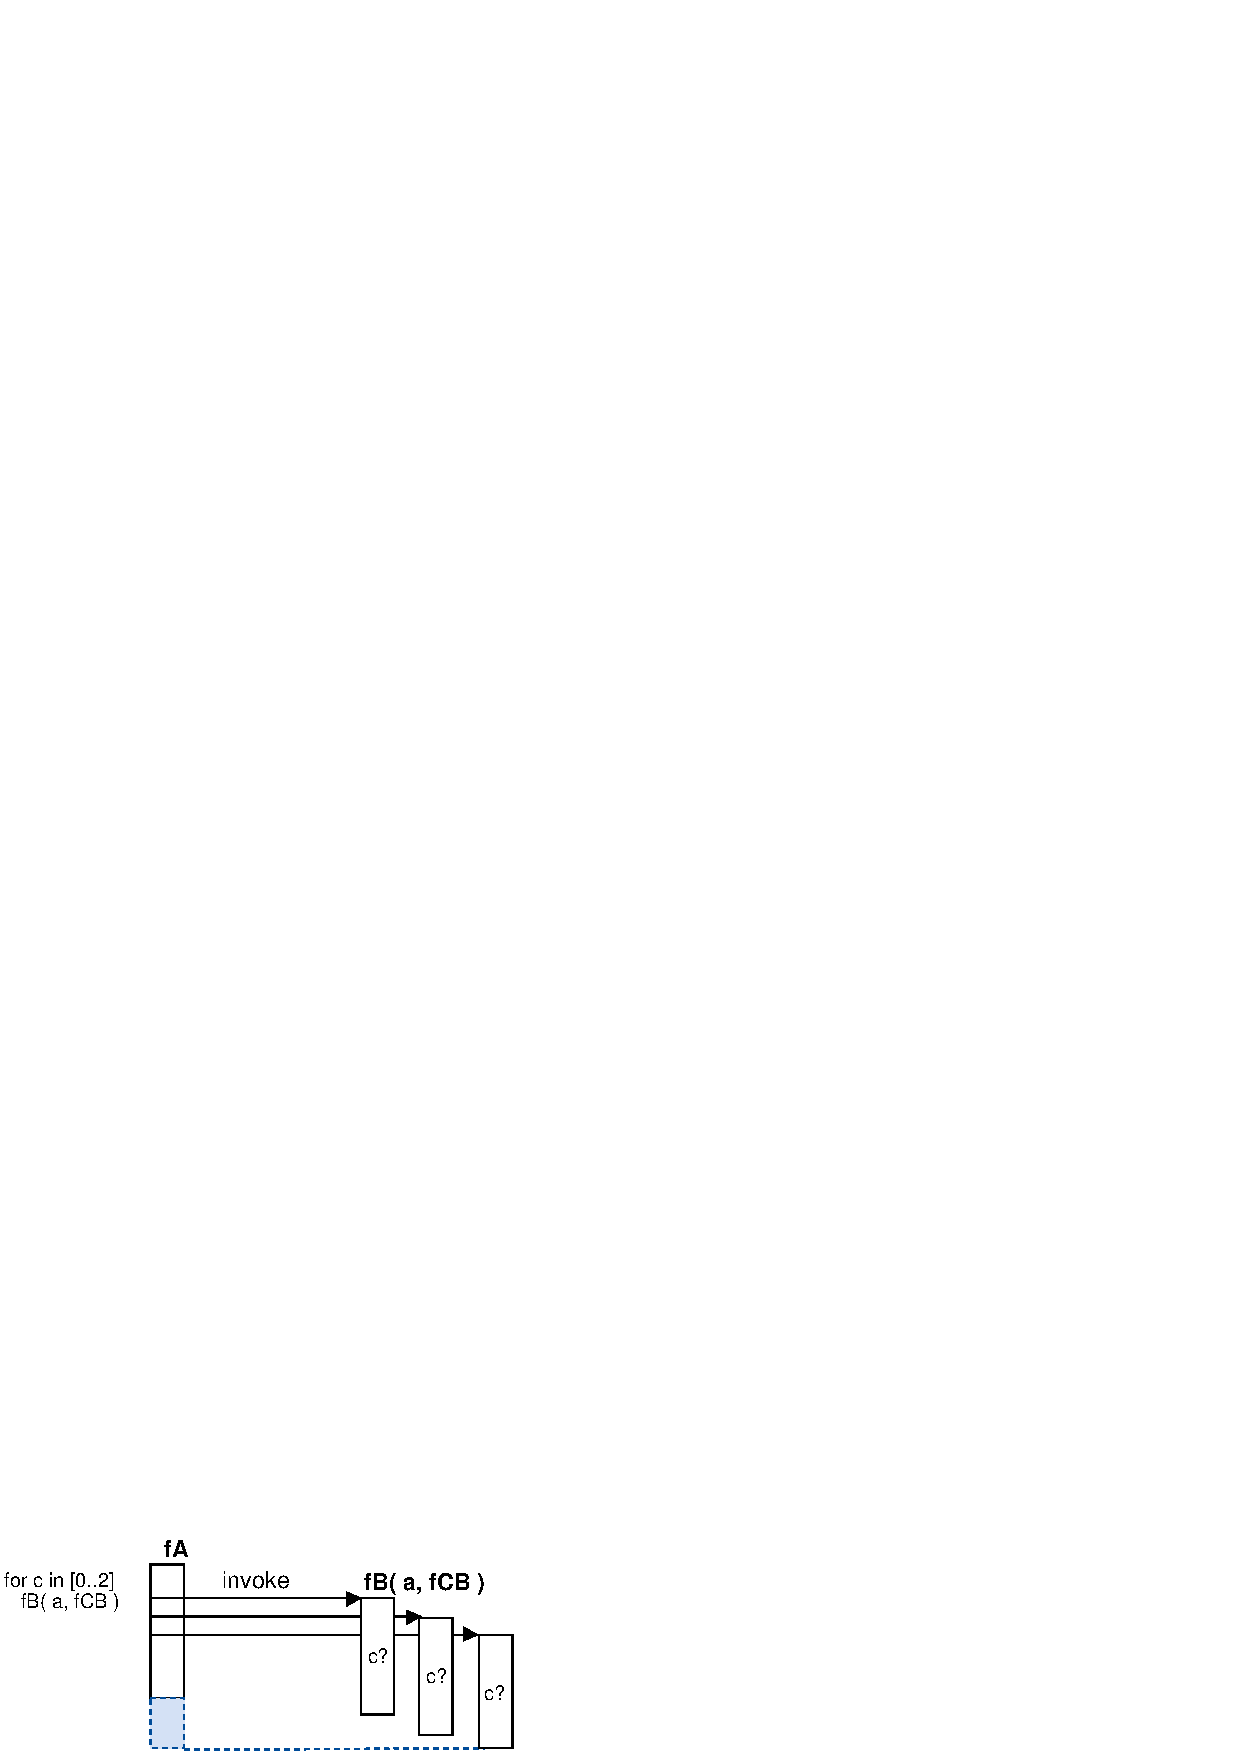
\includegraphics{figures/Closures_Closure-2}
	\caption{Closure context changes in a loop}
	\label{fig:Closures_Closure-2}
\end{figure}


Those event-driven context overwrites can be taken care of by shielding the closure from context changes, as shown in Figure~\ref{fig:Closures_Closure-3}.
To shield the closure form context changes, closure \texttt{fB} needs to create another closure \texttt{fC} and return it to \texttt{fA}.
The argument passed to \texttt{fB} is the context ( \texttt{c} in Figure~\ref{fig:Closures_Closure-3} ) that might change but requires to be persistent for one invocation.
\texttt{fC} has now \texttt{c} as a fixed context, which ca not be overwritten anymore.
Now the only thing left is \texttt{fC} needs to be invoked and it will retain the original context.
This implementation is necessary when the closure acts as a callback function for asynchronous operations, to preserve the original context in case it is required within the callback function.
\begin{figure}[!ht]
	\centering
  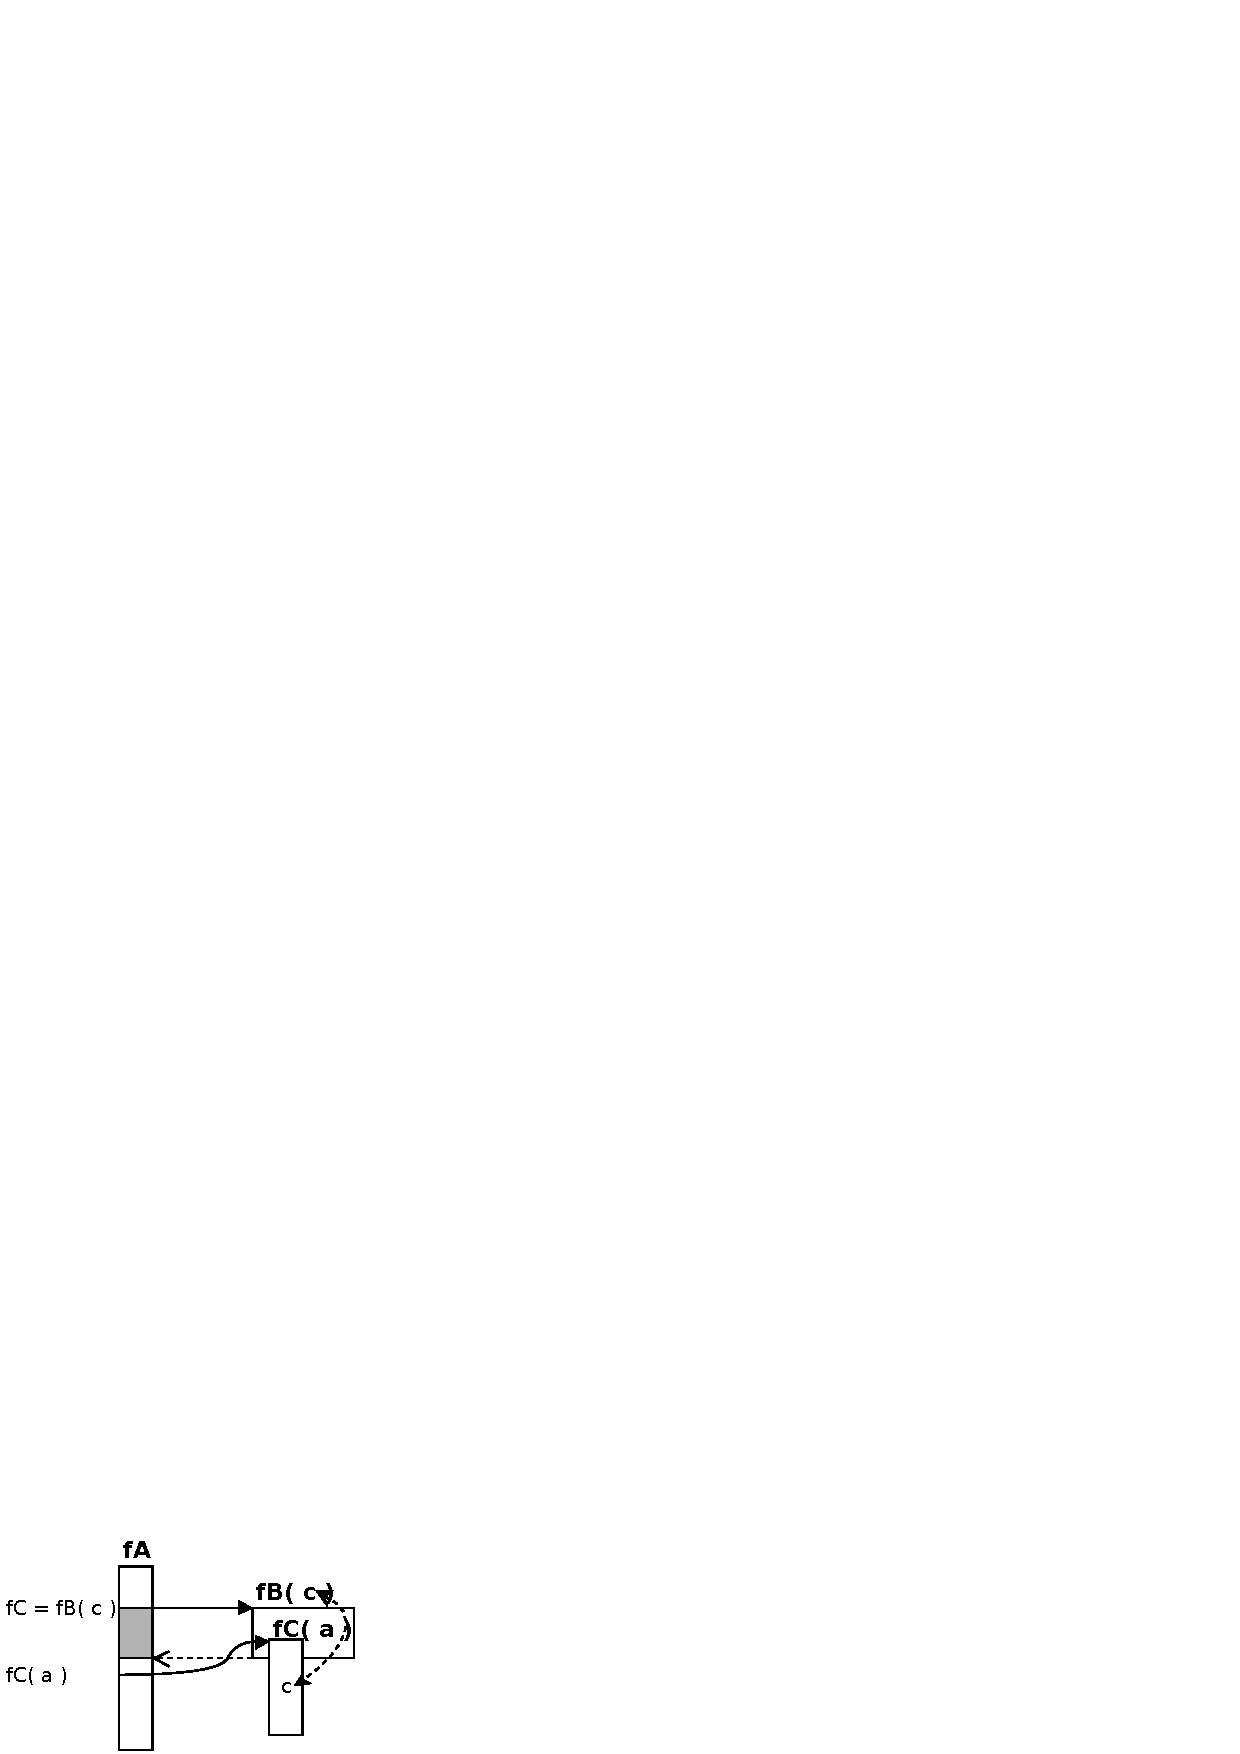
\includegraphics{figures/Closures_Closure-3}
	\caption{Closure Context Shielding}
	\label{fig:Closures_Closure-3}
\end{figure}

% TODO Figures need fA to be right aligned

An example of how closure contexts can be shielded is shown in the Listing \ref{lst_closure}.
\begin{lstlisting}[float=h,label=lst_closure,language=JavaScript,caption=JavaScript Closure Context Shielding]
var fB = function( c ) { // Declare a function...
	var fC =  function( a ) { // ( <-- function to return )
		console.log( c );
	};
	return fC;
};
for( var c = 0; c < 100; c++ ) {
	// ... before you assign it to an event happening in the future:
	var fC = fB( c );
	setTimeout( fC, 3000); // will be executed after the loop ended
}
\end{lstlisting}


